%% LyX 2.0.2 created this file.  For more info, see http://www.lyx.org/.
%% Do not edit unless you really know what you are doing.
\documentclass[british]{article}
\usepackage[T1]{fontenc}
\usepackage[latin9]{inputenc}
\usepackage{geometry}
\geometry{verbose,tmargin=3cm,bmargin=3cm,lmargin=3cm,rmargin=3cm,
headheight=2cm,headsep=3cm,footskip=2cm}
\usepackage{fancyhdr}
\pagestyle{fancy}
\setlength{\parskip}{\bigskipamount}
\setlength{\parindent}{0pt}
\usepackage{babel}
\usepackage{units}
\usepackage{amsmath}
\usepackage{amssymb}
\usepackage{graphicx}
\usepackage{wrapfig}
\usepackage{esint}
\PassOptionsToPackage{normalem}{ulem}
\usepackage{ulem}
\usepackage[unicode=true,
 bookmarks=true,bookmarksnumbered=true,bookmarksopen=true,bookmarksopenlevel=2,
 breaklinks=false,pdfborder={0 0 0},backref=false,colorlinks=false]
 {hyperref}
\hypersetup{pdftitle={Electronics},
 pdfauthor={Josh Wainwright}}

\makeatletter

%%%%%%%%%%%%%%%%%%%%%%%%%%%%%% LyX specific LaTeX commands.
\newcommand{\noun}[1]{\textsc{#1}}
%% Because html converters don't know tabularnewline
\providecommand{\tabularnewline}{\\}

%%%%%%%%%%%%%%%%%%%%%%%%%%%%%% User specified LaTeX commands.
\usepackage{babel}
\usepackage{babel}
\renewcommand{\d}{\mathrm{d}} % for integrals
\newcommand{\dx}[2]{\frac{\textrm{d} #1}{\textrm{d} #2}} % for derivatives
\newcommand{\dd}[2]{\frac{\textrm{d}^2 #1}{\textrm{d} #2^2}} % for double derivatives
\newcommand{\pd}[2]{\frac{\partial #1}{\partial #2}} % for partial derivatives
\newcommand{\pdd}[2]{\frac{\partial^2 #1}{\partial #2^2}} % for double partial derivatives
\renewcommand{\u}[1]{\underline{#1}} % for underline's vectors
\newcommand{\sintertext}[1]{\intertext{#1}\\[-0.7cm]}
\usepackage{mathtools}\hyphenpenalty=50
\usepackage[font=small,labelfont=bf,textfont=it]{caption}





\makeatother

\begin{document}

\title{Electronics}


\author{Josh Wainwright}

\maketitle

\tableofcontents

\part{Overview}
\section{Electronics}

\textbf{Sensor:} Device that measures a physical quantity and converts it into a signal, which can be detected and eventually read by a user, e.g.\ LDR, photomultiplier, thermistor.

There are two types of transducer. First is a sensor, second, and actuator which is a device which converts a signal into some physical effect. For example, a microphone is a sensor, and a loudspeaker is an actuator.

\subsection{Archetypal System}

\begin{minipage}[t]{1\columnwidth}%
\noindent \begin{center}
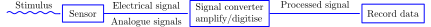
\includegraphics{Electronics/archetypal_system}
\par\end{center}%
\end{minipage}

\begin{minipage}[t]{1\columnwidth}%
\noindent \begin{center}
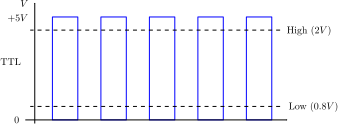
\includegraphics{Electronics/TTL}
\par\end{center}%
\end{minipage}

\subsection{Sensor}
A sensor can be represented by Thevenin's theorem. Thevenin's theorem says that any sensor can be represented by a voltage source and a source impedance.

\begin{minipage}[t]{1\columnwidth}%
\noindent \begin{center}
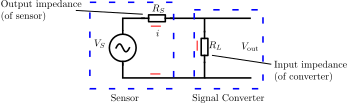
\includegraphics{Electronics/thevenin}
\par\end{center}%
\end{minipage}

\subsection{Impedance Matching}
The sensor signal which is measured is $V_{\text{out}}$ (not $V_S$). Current flowing in the circuit is given by,
\begin{align*}
	i &= \frac{V_S}{R_S+R_L}
\end{align*}
Therefore, the observed signal across the load $R_L$ is
\begin{align*}
	V_{\text{out}} &= iR_L \\
	&= V_S\left(\frac{R_L}{R_S+R_L} \right)
\end{align*}
If $R_L \ll R_S$, then $V_{\text{out}} \ll V_S$. But if $R_L\approx R_S$, then $V_{\text{out}} \approx \frac{1}{2} V_S$

\uline{\noun{Ex}}

Consider the following circuit,

\begin{minipage}[t]{1\columnwidth}%
\noindent \begin{center}
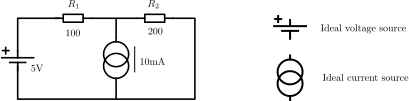
\includegraphics{Electronics/superposition}
\par\end{center}%
\end{minipage}

What is the voltage across $R_{2}$?

\paragraph{Superposition}

Consider the effect of each source separately then add the two effects.

\subsubsection{Voltage Source}

\begin{minipage}[t]{1\columnwidth}%
\noindent \begin{center}
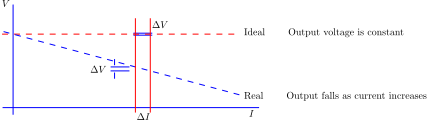
\includegraphics{Electronics/voltage_source}
\par\end{center}%
\end{minipage}

Effective resistance, ${\displaystyle {R=\frac{\Delta V}{\Delta I}}}$.
For the ideal source, $R_{s}=0$ (i.e.\ short circuit)

$\therefore$ Consider the ideal voltage source to have zero internal
resistance.


\subsubsection{Current Source}

\begin{minipage}[t]{1\columnwidth}%
\noindent \begin{center}
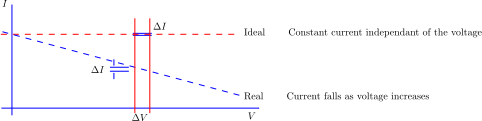
\includegraphics{Electronics/current_source}
\par\end{center}%
\end{minipage}

Effective resistance, ${\displaystyle {R=\frac{\Delta V}{\Delta I}}}$
For the ideal source, $R\rightarrow\infty$. $\therefore$ Take the
current source as having infinite internal resistance (i.e.\ open
circuit).
\begin{enumerate}
\item Consider the effect of just the voltage source by switching the current
source off, so $10\unit{mA}\rightarrow0$ and is replaced by an open
circuit.


\begin{minipage}[t]{1\columnwidth}%
\noindent \begin{center}
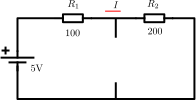
\includegraphics{Electronics/superposition_just_voltage}
\par\end{center}%
\end{minipage}
\item Consider the current source only by switching off the voltage source,
so $5\text{V}\rightarrow0$ and is replaced by a short circuit.


\begin{minipage}[t]{1\columnwidth}%
\noindent \begin{center}
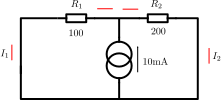
\includegraphics{Electronics/superposition_just_current}
\par\end{center}%
\end{minipage}
\end{enumerate}
Using the superposition principle, we can say that the current through
$R_{2}$ is the sum of these two,
\begin{align*}
I & =\frac{5}{300}+\frac{10}{3}\times10^{-3}\\
 & =\frac{5}{300}+\frac{1}{50}=\frac{6}{300}=\frac{1}{50}\unit{Amps}
\end{align*}
 $\therefore$ Voltage across $R_{2}=\frac{1}{50}\times200=4\unit{V}$.


\subsection{Review of Circuit Components}

The most important three components that a general circuit can be
composed of are the resistor, capacitor and the inductor.
\begin{enumerate}
\item \textbf{Resistance} By Ohm's law, $V_{R}=iR$


\begin{minipage}[t]{1\columnwidth}%
\noindent \begin{center}
\includegraphics{Electronics/resistor}
\par\end{center}%
\end{minipage}
\item \textbf{Capacitance} ${\displaystyle {V_{c}=\frac{q}{C}}}$, where
C is the capacitance given by ${\displaystyle {C=\frac{\epsilon_{0}A}{d}}}$, where $A$ is the area of the capacitor and $d$ is the separation of the plates.


\begin{minipage}[t]{1\columnwidth}%
\noindent \begin{center}
\includegraphics{Electronics/capacitor}
\par\end{center}%
\end{minipage}
Now
\begin{alignat*}{2}
q & =\int i\d{t}\\
\therefore V_{c} & =\frac{\int i\d{t}}{C} & \qquad\text{\noun{Or}}\qquad\dx{V_{c}}{t} & =\frac{i}{C}\\
 &  & \qquad i & =C\dx{V_{c}}{t}
\end{alignat*}
 When $V_{c}$ is constant, $i=0$. Therefore, there is no current
flows through a capacitor when a DC voltage is applied. Therefore,
under DC conditions, the capacitor acts as an open circuit. But current
does flow through a capacitor when the applied voltage across it changes,
\begin{align*}
\because i & =C\dx{V_{c}}{t}
\end{align*}
 When $\dx{V_{c}}{t}$ is large, the current is large. For an infinitesimally
small time interval, $\Delta t$, $\Delta V$ will be very small as
well, but the ratio of $\frac{\Delta V}{\Delta t}$ may be significant.
This implies then that the current, $i$ may be appreciable. But as
usual, the effective resistance, $R=\frac{\Delta V}{\Delta i}$.


For the infinitesimal changes, $\Delta V$ may be small and $\Delta i$
may be large, such that $R\rightarrow0$. Therefore a capacitor will
act as a short circuit when instantaneous changes occur.

\item \textbf{Inductance \textquotedbl{}Choke\textquotedbl{}} An inductor
is a coil of thick wire (so that the resistance, ideally, is zero)
wrapped around a metal core.

\begin{minipage}[t]{1\columnwidth}%
\noindent \begin{center}
\includegraphics{Electronics/inductor}
\par\end{center}%
\end{minipage}

If the current is constant, then $V_{L}=0$. If the current changes,
the magnetic field changes as well,so, by Faraday's Law, there is
an induced electromotive force (back emf),
\begin{align*}
\epsilon & =-\dx{\phi}{t}
\end{align*}
 where $\phi$ is the flux threading the coil. But $\phi\propto i$,
which means
\begin{align*}
\phi & =Li\\
\therefore\epsilon & =-L\dx{i}{t}
\end{align*}

\begin{enumerate}
\item If $i=$ constant, then $V=0$. So the inductor acts as a short circuit
under DC conditions.
\item For infinitesimally small changes, $\Delta t$ will be small and $\Delta i$
will be small also. But again, the ratio, $\frac{\Delta t}{\Delta i}$,
may be significant, and so $\Delta L$ may be significant. The effective
resistance is given by
\begin{align*}
R & =\frac{\Delta V}{\Delta i}\\
 & \approx\frac{\text{finite}}{\text{zero}}\rightarrow\infty
\end{align*}
 Therefore for instantaneous changes, the inductor behaves like an
open circuit.
\end{enumerate}
\end{enumerate}
To summarise,

\begin{center}
\begin{tabular}{l|ccc}
 & \textbf{R}  & \textbf{C}  & \textbf{L} \tabularnewline
\hline
Steady Conditions (DC)  & R  & open circuit  & short circuit \tabularnewline
Instantaneous Changes  & R  & short circuit  & open circuit \tabularnewline
\end{tabular}
\par\end{center}

\section{Time Response}

Consider the time response of an RC circuit. How does the circuit respond to DC conditions and instantaneous changes?

\begin{minipage}[t]{1\columnwidth}%
\noindent \begin{center}
\includegraphics{Electronics/RC_circuit}
\par\end{center}%
\end{minipage}
\begin{enumerate}
	\item \textbf{DC} so the capacitor acts as an open circuit. $\displaystyle{\frac{V_{\text{out}}}{V_{in}}=1}$
	\item \textbf{Instantaneous changes} so the capacitor now acts as a short circuit. $\displaystyle{\frac{V_{\text{out}}}{V_{in}}=0}$
\end{enumerate}
Low frequency signals pass through unimpeded, whereas high frequency signals are blocked. This setup, then, acts as a "low pass" filter.

Consider the same circuit, but with the components swapped.

\begin{minipage}[t]{1\columnwidth}%
\noindent \begin{center}
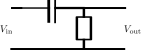
\includegraphics{Electronics/CR_circuit}
\par\end{center}%
\end{minipage}
\begin{enumerate}
	\item \textbf{DC}, the capacitor is still an open circuit, but now $\displaystyle{\frac{V_{\text{out}}}{V_{in}}=0}$
	\item \textbf{Instantaneous changes}, $\displaystyle{\frac{V_{\text{out}}}{V_{in}}=1}$
\end{enumerate}
Now, the low frequency signals are blocked and high frequency signals are unaffected leading to the "high pass" filter.

\subsection{Quantitative Time Response of RC Circuit}
\begin{minipage}[t]{1\columnwidth}%
\noindent \begin{center}
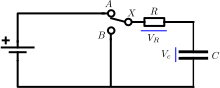
\includegraphics{Electronics/RC_with_switch}
\par\end{center}%
\end{minipage}

Initially, the switch is at A, so $q=0$, $V_R=0$ and $V_c=0$. At time $t=0$, the switch is moved from A to B. At this instant, the capacitor C acts like a short circuit, and so a current flows,
\begin{align*}
	i &= \frac{V}{R}
\end{align*}
And then, by Ohm's law, $V_R=V$ and $V_c=0$. After a long time (under dc conditions) the capacitor acts like an open circuit, and so the current must fall to zero.

By Kirchhoff's laws,
\begin{align*}
	V &= V_R + V_c\\
	&= iR +q\frac{i}{C}
\sintertext{Differentiating this gives}
	0 &= R\dx{i}{t} +\frac{1}{C} \dx{q}{t}\\
	&= R\dx{i}{t} +\frac{1}{C} i \\
	\Rightarrow \int \frac{\d{i}}{i} &= \int \frac{1}{RC} \d{t} \\
	i &= \frac{V}{R} e^{-\frac{t}{RC}}\\
\sintertext{This gives the exponential falloff as expected, and now,}
	\Rightarrow V_R &= iR = V e^{-\frac{t}{RC}} \\
	\Rightarrow V_c &= V-V_R = V \left(1-e^{-\frac{t}{RC}} \right)
\end{align*}

At time $t=0$, the switch is moved from A to B and current flows through the components.

At time $t=t_1$, the switch is moved back from B to A, so the applied voltage falls back to zero. At this instant, no charge moves and therefore, $V_c$ is unchanged. At $t \leqq t_1$,
\begin{align*}
	i &= \frac{V}{R} e^{-\frac{t_1}{RC}} \\
	V_R &= V  e^{-\frac{t_1}{RC}} \\
	V_c &= V\left(1- e^{-\frac{t_1}{RC}}\right)
\end{align*}
At $t \geqq t_1$,
\begin{align*}
	0 &= V_R +V_c \\
	V_R &= -V_c \\
	V_R &= -V\left(1- e^{-\frac{t_1}{RC}}\right)
\end{align*}
At $t=t_1$, $V_R$ changes from $V_R = V\left(1- e^{-\frac{t_1}{RC}}\right)$ to $V_R=-V\left(1- e^{-\frac{t_1}{RC}}\right)$. So the change in $V_R=-V$. 

\begin{minipage}[t]{1\columnwidth}%
\noindent \begin{center}
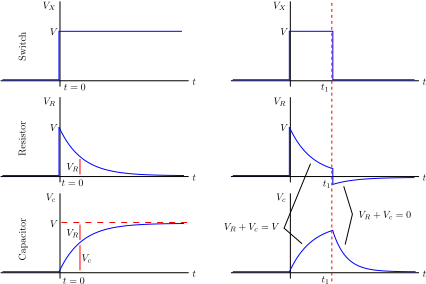
\includegraphics{Electronics/SRC_responce}
\par\end{center}%
\end{minipage}

When the switch is closed, the full change in voltage appears across the resistance.

The low pass filter can be regarded then, as an integrator.
\begin{align*}
	V_{\text{out}} &= V_c = V\left( 1-e^{-\frac{t}{RC}} \right)
\sintertext{For small times, $t \ll RC$,}
	V_{\text{out}} &= V\left( 1- \left(1-\frac{t}{RC}\right) \right) = V\frac{t}{RC}
\end{align*}
Therefore, $V_{\text{out}}$ is approximately the integral of $V_{\text{in}}$ with respect to $t$. Similarly, the high pass filter can be regarded as a differentiator.

\begin{minipage}[t]{1\columnwidth}%
\noindent \begin{center}
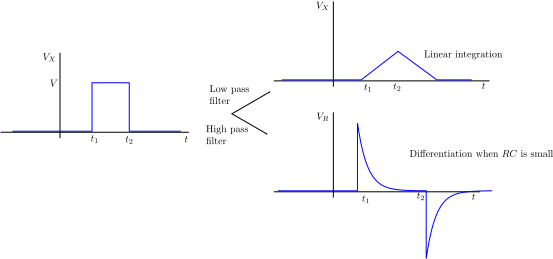
\includegraphics{Electronics/low_integrator_high_differentiator}
\par\end{center}%
\end{minipage}

\subsection{Response to Pulses}
Apply now a train of pulses of time period $T$.
\subsubsection{Low Pass Filter}

\begin{minipage}[t]{1\columnwidth}%
\noindent \begin{center}
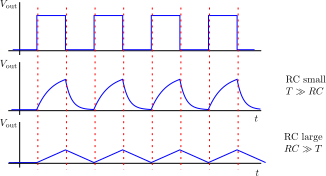
\includegraphics{Electronics/low_pulses}
\par\end{center}%
\end{minipage}

\subsubsection{High Pass Filter}
When the same input pulses are input to $V_{\text{in}}$.

\begin{minipage}[t]{1\columnwidth}%
\noindent \begin{center}
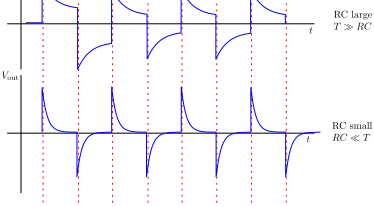
\includegraphics{Electronics/high_pulses}
\par\end{center}%
\end{minipage}

\subsection{Transfer Functions}
\begin{align*}
	V_{\text{out}} &= T\times V_{\text{in}}
\end{align*}
Assume that the current is sinusoidal, such that,
\begin{align*}
	i &= I\sin(\omega t)
\end{align*}
\begin{alignat*}{6}
	V_R &= I_0 R\sin(\omega t) &\qquad V_c &=-\frac{I}{\omega C} \cos(\omega t) & \qquad V_L &=I_0 \omega L \cos(\omega t) \\
	&&&=\frac{I}{\omega C} \sin\left(\omega t -\frac{\pi}{2} \right) &&=I_0 \omega L \sin\left(\omega t + \frac{pi}{2} \right)
\end{alignat*}

\subsection{Phase Differences}

\begin{minipage}[t]{1\columnwidth}%
\noindent \begin{center}
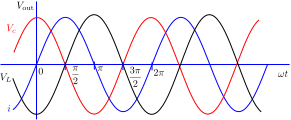
\includegraphics{Electronics/phase_differences}
\par\end{center}%
\end{minipage}
$V_c$ reaches it peak at a later time to $i$ meaning $V_c$ lags behind $i$ by $\frac{\pi}{2}$. $V_L$ reaches its peak at an earlier time, so $V_L$ leads ahead of $i$ by $\frac{\pi}{2}$. There is a dependence of the amplitude on frequency, $\omega$, and there is a phase difference.

\subsection{Move to Complex Notation}

Now the current is given by
\begin{align*}
	i &= I_0 e^{j\omega t} \qquad\qquad j=\sqrt{-1}
\end{align*}
Also
\begin{align*}
	V_R &= I_0 R e^{j\omega t} = iR\\
	V_c &= \frac{I_0}{j \omega C} e^{j\omega t} = \frac{i}{j\omega C} = \frac{i}{\omega C} e^{-j\frac{\pi}{2}} \\
	V_L &= LI_0 e^{j\omega t} = j\omega L i = i\omega L e^{j\frac{\pi}{2}}
\end{align*}
$e^{\pm j\frac{\pi}{2}}$ represents a phase lag and lead respectively of $90^{\circ}$.

Resistance is measured in ohms ($\Omega$) and is real. Impedance is also measured in ohms ($\Omega$) but is complex.
\begin{center}
\begin{tabular}{c|ccc}
	&R&C&L \\ \hline
	Impedance, $Z$ &$Z_R=R$ & $\displaystyle{Z_c = \frac{1}{j\omega C}}$ & $Z_L = j\omega L$
\end{tabular}
\end{center}
So in a circuit, just substitute 
\begin{align*}
	C &\rightarrow \frac{1}{j\omega C} \\
	L &\rightarrow jL\omega
\end{align*}
Then apply Ohm's, Kirchhoff's laws etc.

\subsection{RC Series Circuit as a Single Time Constant Filter}
\begin{align*}
	V_0 &= TV_1
\end{align*}

Potential divider,
\begin{align*}
	T = \frac{V_0}{V_1} &= \frac{Z_c}{Z_c+Z_R} \\
	&= \frac{\frac{1}{j\omega C}}{R+ \frac{1}{j\omega C}} = \frac{1}{1+j\omega CR}
\end{align*}
This is the voltage divider theorem. Any complex number can be expressed as an amplitude and a phase.

Complex Number: $T=a+jb \rightarrow re^{j\phi} \rightarrow r\cos \phi + jr \sin \phi$
\begin{align*}
\left.\begin{array}{c}
	a = r\cos\phi\\
	b = r\sin\phi
\end{array}\right\} r= \left(a^2 + b^2 \right)^{\frac{1}{2}}\\
\end{align*}
\begin{align*}
	\tan\phi &= \frac{\sin\phi}{\cos\phi} = \frac{a}{b}
\end{align*}
Transfer function (complex number) $\rightarrow$ amplitude $+$ phase

\u{\noun{Ex}}
\begin{align*}
	T &= \frac{1-j\omega CR}{(1-j\omega CR)(1+j\omega CR)} \\
	&= \frac{1-j\omega CR}{1+(\omega CR)^2} = A e^{i \phi}
\sintertext{where $A$ is the amplitude and $\phi$ is the phase.}
	A &= \left[ \left(\frac{1}{1+(\omega CR)^2} \right)^2 +\left(\frac{\omega CR}{1+(\omega CR)^2} \right) \right]^{\frac{1}{2}} \\
	&= \frac{1}{(1+(\omega CR)^2)^{\frac{1}{2}}}\\
	\tan\phi &= -\omega CR
\end{align*}
These data could be plotted linearly, but it is much more useful and easier to interpret if they are plotted on a double log plot, called a Bode plot.

\subsection{Bode Plots}

Bode plots exploit the complex impedance and involves simply plotting $\log_{10}(|T|)$ against $\log_{10}(\omega)$ or $\phi$ against $\log_{10}(\omega)$. The transfer function is defined as the output voltage divided by the input voltage, and is also complex.

When plotted in this way, the Bode plot is almost exactly two straight lines. There is a small amount of error at the connection of these lines since there should be a small amount of curvature here.

\subsubsection{Decibels}
Decibels are used to represent power ratios between two signals. For voltages,

\begin{minipage}{0.7\textwidth} 
\begin{align*}
	\text{dB} &= 20\log_{10}\left(\frac{V_2}{V_2}\right)
\sintertext{and for powers,}
	\text{dB} &= 10 \log_{10} \left(\frac{P_2}{P_2}\right)
\sintertext{since}
	P &= \frac{V^2}{R}
\end{align*}
\end{minipage} 
\hspace{0.5cm} 
\begin{minipage}{0.4\linewidth}
	\begin{center}
		\begin{equation*}
			\begin{array}{c|c}
				\frac{V_2}{V_1} & \text{dB} \\ \hline \hline
				1000 & 60 \\
				100 & 40 \\
				10 & 20 \\
				-\sqrt{2} & 3.01 \\
				1 & 0 \\
				\frac{1}{\sqrt{2}} & -3.01 \\
				0.1 & -20 \\
				0.01 & -40 \\
				0.001 & -60
			\end{array}
		\end{equation*}
	\end{center}
\end{minipage}

When $|T|=20\log_{10}\left(\frac{V_{\text{out}}}{V_{\text{in}}}\right) = -3$dB. This represents when the power has been reduced by a factor of 2. This occurs when $\omega=\omega_0$ and so $\omega_0$ is called the half power frequency, or $-3$dB frequency.

\u{\noun{Ex}}

High pass filter,
\begin{itemize}
	\item Express the transfer function as a complex number,
	\begin{align*}
		T &= \frac{V_0}{V_1} =\frac{iR}{V_i} = \frac{R}{V_i}\frac{V_i}{R+\frac{1}{j\omega C}} \\
		&= \frac{R}{R+\frac{1}{j \omega C}} = \frac{Rj\omega C}{1+Rj\omega C}
	\end{align*}
	when $\omega \rightarrow \infty,\; T\rightarrow 1$ and when $\omega \rightarrow 0, \; T\rightarrow 0$, which is the usual high pass filter results, as expected.
	\item Express T as an amplitude, $|T|$, and a phase, $\phi$.
	\begin{align*}
		T &= \frac{Rj \omega C}{1+Rj \omega C} \times \frac{1-Rj \omega C}{1-Rj \omega C} \\
		&= \frac{j\omega CR+\omega^2 C^2 R^2}{1+\omega^2 C^2 R^2} \\
		\Rightarrow |T| &= \frac{\left((\omega^2 C^2 R^2)^2 + \omega^2 C^2 R^2 \right)^{\frac{1}{2}}}{1+ \omega^2 C^2 R^2} \\
		&= \frac{\omega CR}{(1+\omega^2 C^2 R^2)^{\frac{1}{2}}}
	\end{align*}
	So as $\omega \rightarrow \infty, \; |T|\rightarrow 1$, as $\omega \rightarrow 0, \; |T|\rightarrow 0$ and as $\omega \rightarrow \omega_0, \; |T|\rightarrow \frac{1}{\sqrt{2}}\; (-3\text{dB})$
	Phase difference between $V_0$ and $V_1$ is $\phi$,
	\begin{align*}
		\phi &= \tan^{-1}\left( \frac{\Im\{ T\}}{\Re \{T\}}\right) \\
		&= \tan^{-1}\left( \frac{\omega CR}{\omega^2 C^2 R^2}\right) = \tan^{-1}\left( \frac{1}{\omega CR}\right)
	\end{align*}
	when  $\omega \rightarrow \infty, \; \phi \rightarrow 0$, $\omega \rightarrow \omega_0=\frac{1}{CR}, \; \phi \rightarrow 45^{\circ}$ and $\omega \rightarrow 0, \; \phi \rightarrow 90^{\circ}$
\end{itemize}
Using these Bode plots, the more complex functions can be analysed simply by adding the phase shifts and amplitudes.

\subsubsection{Cascading Transfer Functions}
$V_2$ is both the output of $T_1$ and the input of $T_2$. If $T=T_1 \times T_2$, then
\begin{align*}
	\log_{10} T &= \log_{10} T_1 + \log_{10} T_2
\end{align*}
Therefore, to multiply the transfer functions, add the decibels of $|T_1|$ and $|T_2|$.

\subsubsection{Phases}
\begin{align*}
	T_1 &= a+ jb \\
	T_2 &= p+jq \\
\sintertext{If}
	T &= T_1T_2 \\
	&= (a+jb)(p+jq) \\
	&=(ap-bq)+j(bp+aq) \\
	\Rightarrow \phi &= \tan^{-1} \left(\frac{bp+aq}{ap-bq} \right)
\sintertext{But}
	\tan(\phi_1 +\phi_2) &= \frac{\tan \phi_1 +\tan \phi_2}{1- \tan\phi_1 \tan\phi_2} \\
	&= \frac{b/a - q/p}{b/a \times q/p} \\
	\phi &= \phi_1 + \phi_2
\end{align*}
When the transfer functions are multiplied, the phases are added together.

\u{\noun{Ex}}
Example of cascading transfer functions


The circuit is an effective high pass filter, but at low frequencies, the phase difference is $-180^{\circ}$ so the output is a negative multiple of the input.

\subsubsection{Generalised Function}
Any transfer function, $T(\omega)$ can be expressed as,
\begin{align*}
	T &= K\frac{\left( 1+\frac{j\omega}{Z_1} \right)+\left( 1+\frac{j\omega}{Z_n} \right)+\ldots +\left( 1+\frac{j\omega}{Z_n} \right)}{\left( 1+\frac{j\omega}{P_1} \right)+\left( 1+\frac{j\omega}{P_2} \right)+\ldots+\left( 1+\frac{j\omega}{P_n} \right)}
\end{align*}
where $K$ is a multiplicative constant, $Z_n$ are transfer-function zeroes and $P_n$ are transfer-function poles. To draw the Bode plot we draw the asymptotes for each zero and each pole and then add the various contributions.

\begin{itemize}
	\item At every value of $\omega=Z_i$, the slope of the line increases by 20dB per decade and at every value of $\omega=P_i$ the slope of the line decreases by 20dB per decade. 
	\item To correct a straight line Bode plot, at every zero, put a point 3dB above the line and at every pole put a point 3dB below the line.
	\item If $K$ is positive, then the zero slope start line will be at 0 degrees, whereas if $K$ is negative, then the start line will be at 180 degrees.
	\item At every value of $\omega=Z_i$ increase the slope of the line by 45 degrees per decade, beginning one decade below $\omega=Z_i$ and ending one decade above $\omega=Z_i$.
	\item At every value of $\omega=P_i$ decrease the slope of the line by 45 degrees per decade, beginning one decade before $\omega=P_i$ and ending one decade above $\omega=P_i$.
\end{itemize}

\part{Operational Amplifiers}
\section{Op-amp Characteristics}
The op-amp is a versatile building block in analogue electronic circuits. It was originally used to perform mathematical operations in analogue computers but are now included in a huge number of different applications because they are so cheap, easy to incorporate and perform very well under a vast range of conditions.

An IC op-amp (e.g.\ 741) consists of around 24 transistors, several resistors and a capacitor. We will not study transistors, so will treat the op-amp as a black box single unit.

\subsubsection{Op-Amp Terminal}
The op-amp has two input and one output terminals. It senses the difference between the voltages at its inputs, $V_+-V_-$, and then multiplies this by a gain, $A$. The output, then becomes
\begin{align*}
	v_0 &= a(v_+ -v_-)
\end{align*}
All of the voltages are measured with respect to ground.

\subsubsection{Ideal Properties}
\begin{itemize}
	\item The op-amp will be considered as an ideal component, meaning it draws no current through any of the input terminals, i.e.\ it has an infinite input impedance.
	\item The output is an ideal voltage source so has zero output impedance.
	\item It has infinite differential gain ($A\rightarrow\infty$) at all frequencies in the range $0\leq \omega \leq \infty$.
\end{itemize}
Zero output impedance means that any amount of current can be taken without changing the voltage. This current cannot come from the inputs as they draw no current. Most IC op-amps require dc power to be supplied (not usually shown). Note that the $+$ and $-$ supplies have nothing to do with the $+$ and $-$ inputs.

\begin{minipage}[t]{1\columnwidth}%
\noindent \begin{center}
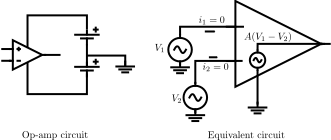
\includegraphics{Electronics/op-amp_circuit_equivalent}
\par\end{center}
\end{minipage}

The op-amp is a differential-input, single-ended-output and is only sensitive to voltage difference, any common signal is ignored. This property is called common-mode rejection. An ideal op-amp has infinite common-mode rejection. Op-amps are direct-coupled devices (amplifies signals whose frequency is as low as $\omega = 0$). The gain $A$ is called the differential gain, or open-loop gain which is ideally infinite. They are never (rarely) used without feedback. Though this reduces the gain, it provides other benefits.

\section{Op-Amp Golden Rules}
\begin{itemize}
	\item The open loop gain $(A)$ is so high that a fraction of a milli-volt difference between the inputs will cause the output to reach maximum value (e.g.\ $\pm 15$V of the power supply) So if the output signal is in the required range (i.e. $\pm 15$V) , then it implies that the two inputs must be at the same value.

	This then means that the voltage difference between the inputs is effectively zero.

	\item The op amp draws negligible current into the inputs, so no current flows into the device what ever voltage is drawn.
\end{itemize}

\section{Applications}
The op-amp is invariably used with feedback, in particular, negative feedback.
\subsection{The Inverting Configuration}

\begin{minipage}[t]{1\columnwidth}%
\noindent \begin{center}
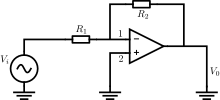
\includegraphics{Electronics/inverting_op-amp}
\par\end{center}
\end{minipage}

The resistor R2 provides negative feedback. The output is fed back to the inverting terminal. The closed loop gain, G, of this configuration can be calculated as follows,
\begin{align*}
	G &=\frac{V_0}{V_i}
\sintertext{From the op-amp equation,}
	V_2 - V_1 &= \frac{V_0}{A} \approx 0
\sintertext{The current in $R_1$ is,}
	i_1 &= \frac{V_i-V_1}{R_1} \approx \frac{V_i}{R_1}
\sintertext{But the op-amp draws no current, so $i_2 = i_1$}
	V_0 &= 0-i_1R_2 \\
	\Rightarrow G &= \frac{V_0}{V_i} = -\frac{R_2}{R_1}
\end{align*}
The inverting amplifier has an input impedance given by
\begin{align*}
	Z_i &= \frac{v_i}{i_1} = \frac{v_i}{v_i/R_1} = R_1
\sintertext{and an output impedance of}
	Z_0 &= 0
\end{align*}
The ap-amp acts like an ideal voltage source.

\subsubsection{Inverting Op-Amp Observations}
\begin{itemize}
	\item The feedback resistor R2 closes the loop around the op-amp, hence G is known as the closed loop gain.
	\item The closed-loop gain is dependent on R1 and R2 only
	\item Gain can be chosen, and made as accurate as you like. The closed-loop gain is smaller than the open-loop gain, but is is stable and predictable
	\item A consequence of the large (ideally infinite) open-loop gain is that the two input terminals track each other in potential.
	\item We speak of a virtual short-circuit between the input terminals. Don't make the mistake of actually shorting them though.
	\item This means that because the non-inverting terminal is grounded, the inverting terminal is a virtual ground.
\end{itemize}

\subsection{The Non-Inverting Configuration}

\begin{minipage}[t]{1\columnwidth}%
\noindent \begin{center}
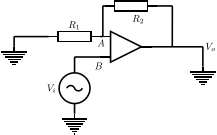
\includegraphics{Electronics/non-inverting_amp}
\par\end{center}
\end{minipage}
We can find the closed loop gain (or transfer function) $G$,
\begin{alignat*}{3}
\sintertext{From the op-amp equation}
	V_2-V_1 &= \frac{V_0}{A} \approx 0 &\qquad A\rightarrow \infty, \; V_1\rightarrow V_2
\sintertext{Current in $R_1$}
	i_1 &= \frac{0-V_i}{R_1} = -\frac{V_i}{R_1} &\qquad V_2=V_1 \rightarrow V_1\rightarrow V_i
\sintertext{The op-amp draws no current, so}
	i_2 &= i_1 \qquad V_0 = V_i-i_1R_2 \\
	\Rightarrow G &= \frac{V_0}{V_i} = 1+\frac{R_2}{R_1}
\end{alignat*}
The input impedance is given by
\begin{align*}
	Z_i &= \frac{V_i}{i} = \frac{V_i}{0} = \infty
\sintertext{So the op-amp draws no current. The output impedance is given by}
	Z_0 &= 0
\sintertext{So the op-amp acts like an ideal voltage source.}
\end{align*}

\subsubsection{Non-Inverting Op-Amp Observations}
\begin{itemize}
	\item Once again, the closed loop gain is dependant only on $R_1$ and $R_2$, not on the properties of the op-amp itself.
	\item The closed loop gain is positive, hence non-inverting, so the output is in phase with the input.
	\item A consequence of the large (ideally infinite) open-loop gain is that the two terminals track each other in potential, as before. 
	
	This means that the non-inverting terminal is at the same potential as the inverting terminal, which is the applied voltage.
	\item Note that the inverting terminal cannot be connected directly to the ground, and this also assumes that the op-amp is working, i.e.\ the output is not saturated.
\end{itemize}

\subsection{Unity Gain Buffer}
The unity gain buffer, or voltage follower, has unity gain, so does not seem to be useful. Though is has a range of applications since it changes impedance.

\begin{minipage}[t]{1\columnwidth}%
\noindent \begin{center}
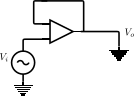
\includegraphics{Electronics/unity_gain_buffer}
\par\end{center}
\end{minipage}
Let $R_1 \rightarrow \infty$, so 
\begin{align*}
	G &= \frac{V_0}{V_1} = 1 + \frac{R_2}{R_1} \rightarrow 1
\end{align*}
This means that the input impedace of the ideal unity-buffer $Z_i = \infty$ so does not load the source. This is particularly useful for weak signals. Also $Z_0=0$ so provides alot of current witout attenuating the signal.






















\end{document}
